% This file (thesis-main.tex) is the main file for a master's thesis.
\documentclass {udthesis}
% preamble

% Include graphicx package for the example image used
% Use LaTeX->PDF if including graphics such as .jpg, .png or .pdf.
% Use LaTeX->PS->PDF if including graphics such as .ps or .eps
% Best practice to not specify the file extension for included images,
% so when LaTeX is building it will look for the appropriate image type.
\usepackage{graphicx}
\usepackage{cite}
\usepackage{algorithmic}
\usepackage{algorithm}
\usepackage{siunitx}
\usepackage{subscript}
\usepackage{flexisym}
\usepackage{hyperref}
%\usepackage{tikz}
\DeclareSIUnit\Molar{\textsc{m}}
\DeclareSIUnit\Units{\textsc{u}}
\begin{document}
%					THESIS - TAP ( T I T L E  +  A P P R O V A L )
% 
% This is the Title and Approval Page file (thesis-tap.tex) for
% a master's thesis.
%
% The order of the commands below is very important.
% You may choose to add or eliminate a \prefacesection 
% in the front material but the order should remain 
% the same especially \maketocloflot followed by 
% \prefacesectiontoc{Abstract}

% Title and author are also used for PDF file properties
% No special character or commands can be used for the PDF definition; 
% use the [options] paramater to specify a different title or author 
% to remove special characters or commands like \\ for example.
\title[Investigating transcriptomic responses to biofuel stress in Clostridium Aceotbutylicum : Transcriptome assembly and genome annotation of a model fermentative bacterium.]{Investigating transcriptomic responses to biofuel stress in \textit{Clostridium acetobutylicum}:\\ Transcriptome assembly and genome annotation of a model fermentative bacterium.}
\author{Matthew T. Ralston}
\type{thesis}
\degree{Master of Science}
\majorfieldtrue\majorfield{Bioinformatics and Computational Biology}
\degreedate{Summer 2014}
% Optional PDF properties
\keywords{Transcriptome,RNA-seq,Assembly,Genomics}
\subject{Master of Science in Bioinformatics and Computational Biology}

\maketitlepage % Generates Title Page

\begin{approvalpage}
\prof{Eleftherios T. Papoutsakis, Ph.D.}
\chair{Errol Lloyd, Ph.D.}{Chair of the Department of Computer Science}
\dean{Babatunde Ogunnaike, Ph.D.}{Dean of the College of Engineering}
\end{approvalpage}

\begin{front} % Starts front material (Roman style page numbers)

\prefacesection{Acknowledgments}

%					A C K N O W L E D G E M E N T S
% Acknowl.tex

I write this paper with unending thanks for my family, friends, the love, support and encouragement that they give, and the lessons they have taught me. With special thanks for my mother Donna, father Thomas, and sister Allison. With special thanks to my mother; her character and duty towards others is inspirational for this work's focus on sustainability and climate change. With special thanks to my Father, for inspiration through his work ethic, leadership, and open mind. With special thanks to my sister for her support of my education, curiosity, and maturity; I would not be where I am without her encouragement and acceptance. I write this with gratitude to my family for the life they have given me, the sacrifices they have made on my behalf, and most importantly their love. With special thanks for my grandfather George inspiring my pursuit of science and chemistry. With special thanks for my grandmother Winnie for the inspiration of her love and optimism which bring me through each challenge. With special thanks for my uncle Kevin for his curiosity, friendship, optimism, and support. With special thanks for my brother-in-law Matt for his friendship and encouragement. With special thanks for my nieces Violet and Ruby for their love, for the lessons that they teach me, and their infectious energy and optimism. Many thanks for Madeline for her love, open ear, curiosity, support, and encouragement throughout the years.  Many thanks to my best friend Andrew for his friendship, curiosity, support, and encouragement. With many thanks to the rest of my wonderful and supportive family and friends for their unconditional love and support. 

Many thanks to Karol Miaskiewicz for his consistent and wonderful friendship throughout this project. Many thanks to all of the members of the Bioinformatics program. Particularly, I'd like to thank Erin Crowgey for her mentorship and support of my efforts to learn NGS bioinformatic analyses and Ryan Moore for tossing ideas around together. I'd like to thank Shawn Polson for his open ear and perspective. I'd also like to thank Dr. Wu for her support and encouragement throughout the program and the many members of the Wu group for their support as well. Many thanks to Bruce, Olga, and Summer for their work in the Sequencing and Genotyping Center in support of this project.

Many thanks for my mentors, Drs. Keerthi Venkataramanan and Terry Papoutsakis, for their mentorship, support, critique, and understanding throughout this project. The success that we've seen in this effort I owe to Keerthi's guidance and training. 
Many thanks for each of the the many members of the Papoutsakis lab for their friendship, support, and critique. I am very grateful for the unity of this group and for how much I enjoy coming to the lab each day. For the hard work, sleepless nights, early autoclave cycles, shared spaces, and plenty of reasons to celebrate I am grateful for each member.

{\centerline {\it Ad maiorem dei gloriam.}} % This file (acknowl.tex) contains the text
                % for the acknowledgments.


% Table of Contents is always created, but you
% may set \tablespagefalse and \figurespagefalse 
% if you don't want these generated automatically
% (i.e. List of Tables and List of Figures).
% These are set to true by default (i.e. \tablespagetrue,
% \figurespagetrue).

% Uncomment if you do not want a List of Figures.
%\figurespagefalse

% Uncomment if you do not want a List of Tables.
%\tablespagefalse 

\maketocloflot

\prefacesectiontoc{Abstract}

%					A B S T A C T
%% Abstract.tex


The {\it C. acetobutylicum} genome annotation has been markedly improved by integrating bioinformatic predictions with RNA sequencing(RNA-seq) data. Analysis of an initial assembly revealed errors due to technical and biological background signals, challenges with few solutions in the genomic literature. Additional hurdles for next-generation sequencing(NGS) based transcriptome mapping research include optimizing library complexity and sequencing depth, yet most studies in bacteria report low depth and ignore the effect of ribosomal RNA abundance and other sources on the effective sequencing depth. 

In this work, \textit{in vitro} and \textit{in silico} workflows were established to address false positive and negative errors associated with transcriptome mapping. An integrative analysis method was developed to integrate motif predictions, single-nucleotide resolution sequencing depth, and complexity during curation. This contextualization minimized false positive error, providing the precise and accurate determination of gene boundaries qualitifed by previous studies, in some cases, to the exact basepair. Curation of the pSOL1 megaplasmid improved statistical measures of transcriptomic features to be amenable with findings from \textit{E. coli}. 

The resulting annotation can be readily explored and downloaded through a customized genome browser, enabling future genomic and transcriptomic research in this organism. This work demonstrates the first strand-specific transcriptome assembly in the \textit{Clostridia}. Additionally, this method can be used to eliminate false positive features from assemblies in bacterial transcriptome mapping studies.  % This file (abstract.tex) contains the text
                 % for an abstract.
% Abstract.tex


The {\it C. acetobutylicum} genome annotation has been markedly improved by integrating bioinformatic predictions with RNA sequencing(RNA-seq) data. Analysis of an initial assembly revealed errors due to technical and biological background signals, challenges with few solutions in the genomic literature. Additional hurdles for next-generation sequencing(NGS) based transcriptome mapping research include optimizing library complexity and sequencing depth, yet most studies in bacteria report low depth and ignore the effect of ribosomal RNA abundance and other sources on the effective sequencing depth. 

In this work, \textit{in vitro} and \textit{in silico} workflows were established to address false positive and negative errors associated with transcriptome mapping. An integrative analysis method was developed to integrate motif predictions, single-nucleotide resolution sequencing depth, and complexity during curation. This contextualization minimized false positive error, providing the precise and accurate determination of gene boundaries qualitifed by previous studies, in some cases, to the exact basepair. Curation of the pSOL1 megaplasmid improved statistical measures of transcriptomic features to be amenable with findings from \textit{E. coli}. 

The resulting annotation can be readily explored and downloaded through a customized genome browser, enabling future genomic and transcriptomic research in this organism. This work demonstrates the first strand-specific transcriptome assembly in the \textit{Clostridia}. Additionally, this method can be used to eliminate false positive features from assemblies in bacterial transcriptome mapping studies. 

\end{front}



                   % This file (thesis-tap.tex) contains the Title
                   % and Approval Page information for a master's thesis.

%					C H A P T E R   1 - Introduction

%%
% This is Chapter 1 file (chap1.tex)
%
\chapter{Title of Chapter}
This is the information for the first chapter, Chapter 1.  Copy the base file, chap1.tex, for additional chapter needed such as chap2.tex, chap3.tex, etc. Modify the main base file to include each additional chapter file.

\section{Title of Section}

This is the information for the first section of the first chapter.    % This file (introduction.tex) contains the text
                   % for Chapter 1- the introduction
                   
%					C H A P T E R   2 - Methods
% This is the Chapter 2 - Methods file (chap2.tex)

\chapter{Methods}


\section{Culture}
Wild type \textit{Clostridium acetobutylicum} ATCC 824 was cultured anaerobically in 4L New Brunswick Scientific BioFlo 310 bioreactors at \SI{37}{\degreeCelsius}, pH >5.0, \SI{200}{\milli\liter\per\minute} N\textsubscript{2} and 200rpm agitation in a defined \textit{Clostridia} growth medium, as described previously (Venkataramanan 2013). When the cultures were grown to A\textsubscript{600}=1, the N\textsubscript{2} flow rate was decreased to \SI{50}{\milli\liter\per\minute} and cultures were either stressed to a final concentration of \SI{60}{\milli\Molar} \textit{n}-butanol, \SI{40}{\milli\Molar} potassium butyrate, or left unstressed. \SI{15}{\milli\liter} samples were acquired at 15, 75, 150, and 270 minutes after treatment and synchronization. Samples were centrifuged at 8,000rpm, \SI{4}{\degreeCelsius} for 20 minutes. After discarding the supernatant, cell pellets were then immediately frozen at \SI{-85}{\degreeCelsius}.

\section{RNA preparation}
RNA was extracted by first washing the cell pellets in 1mL of RNase-free SET buffer (25\% sucrose, \SI{50}{\milli\Molar} EDTA [pH 8.0], \SI{50}{\milli\Molar} Tris-HCl [pH 8.0]) before resuspending cells in a \SI{220}{\milli\liter} solution of RNase-free SET buffer containing \SI{4.55}{\Units\per\milli\liter} proteinase K and \SI{20}{\milli\gram\per\milli\liter} lysozyme and incubating for 6 minutes. Resuspended cells were vortexed with 40mg of RNase-free glass beads ($\leq$\SI{106}{\micro\metre}) at maximum speed and room temperature for 4 minutes. Each sample was mixed immediately with \SI{1}{\milli\liter} of ice-cold QIAzol (Qiagen, Valencia, CA, USA) and then \SI{200}{\micro\liter} of ice-cold chloroform, mixing well. After a 3 minute room temperature incubation, samples were centrifuged at 11,000rpm and \SI{4}{\degreeCelsius} for 15 minutes. The aqueous phase was then mixed with \SI{1.3}{\milli\liter} of ice-cold ethanol before transfering to a miRNeasy Mini spin-column (Qiagen, Valencia, CA, USA) and centrifuging at 11,000rpm and \SI{4}{\degreeCelsius} for 15 seconds.

Next, \SI{700}{\micro\liter} of RWT buffer was added to the column, before centrifuging at 11,000rpm and \SI{4}{\degreeCelsius} for 15 seconds, discarding the collection tube and transferring the column to a fresh collection tube. The column was washed twice with \SI{500}{\micro\liter} of RPE buffer before centrifuging at 11,000rpm and \SI{4}{degreeCelsius} for 15 seconds each. The membrane was then dried with an additional centrifugation step at 11,000rpm and \SI{4}{degreeCelsius} for 1 minute. The RNA was eluted twice by incubating with \SI{50}{\micro\liter} of nuclease-free water for 1 minute and eluting for 1 minute at 11,000rpm and \SI{4}{degreeCelsius}.

After quantification on a Nanodrop ND-1000, samples were then precipitated in 0.3M sodium acetate and 75\% ethanol overnight, centrifuged at 14,000 rpm for 30 minutes, washed twice with \SI{400}{\micro\liter} ice-cold 70\% ethanol, and rehydrated in \SI{50}{\micro\liter} RNase-free water. Next, samples were treated with the Turbo DNA-free kit (Ambion, Austin, TX, USA). \SI{5}{\micro\liter} of 10X Turbo DNase buffer and \SI{1}{\micro\liter} of Turbo DNase (2U\SI{}{\per\micro\liter}) were added to each sample before incubating at \SI{37}{degreeCelsius} for 30 minutes. Next, \SI{5}{\micro\liter} of DNase inactivation reagent were added to each sample, mixing occasionally for 5 minutes. The samples were then centrifuged at 10,000rpm and \SI{4}{degreeCelsius} for 90 seconds, precipitating the DNase. 

Samples were then precipitated, washed twice more with 70\% ethanol, and resuspended in \SI{20}{\micro\liter} of nuclease-free water, requantified, and aliquoted for quality analysis with the BioAnalyzer platform (Agilent, Wilmington, DE, USA), and \SI{10}{\micro\gram} aliquots in \SI{10}{\micro\liter} samples were stored at \SI{-85}{\degreeCelsius}.

\section{RNA enrichment, RNA-seq library preparation, and Sequencing}
Ribosomal RNA was removed with the MicrobExpress kit (Ambion, Austin, TX, USA) according to their protocol. Briefly, beads were prepared by taking \SI{50}{\micro\liter} for each sample, washing with an equal volume (\SI{50}{\micro\liter}) of water capturing for 5 minutes on a MagnaSphere (Promega, Madison, WI, USA) magnetic stand and aspirating. Subsequently, the beads were resuspended in an equal volume (\SI{50}{\micro\liter} each) of binding buffer and capturing as above. The beads were then resuspended in an equal volume (\SI{50}{\micro\liter} each) of binding buffer and warmed to \SI{37}{\degreeCelsius}. Next, \SI{200}{\micro\liter} of binding buffer was added to each \SI{10}{\micro\gram} RNA aliquot with \SI{4}{\micro\liter} of capture oligo mix. The mixture was warmed to \SI{70}{\degreeCelsius} for 10 minutes, then cooled to \SI{37}{\degreeCelsius} for 15 minutes. Next, the rRNA was captured by mixing \SI{50}{\micro\liter} of beads with each sample, incubating for 15 minutes at \SI{37}{\degreeCelsius}, and capturing as above. The enriched RNA was transferred to a fresh \SI{1.5}{\milli\liter} tube. The beads were then washed with \SI{100}{\micro\liter} of pre-warmed (\SI{37}{\degreeCelsius}) wash solution, incubating on the magnetic stand for 5 minutes, and adding the wash solution to the enriched RNA. The samples were then ethanol precipitated at \SI{20}{\degreeCelsius} overnight with \SI{35}{\micro\liter} of \SI{3}{\Molar} Sodium Acetate, \SI{5}{\milli\gram\per\milli\liter} Glycogen, and \SI{1175}{\micro\liter} of chilled 100\% ethanol. The samples were washed twice with 70\% ethanol and resuspended in \SI{25}{\micro\liter}. The samples were enriched further by repeating the MicrobExpress treatment. Small 10-\SI{100}{\nano\gram} aliquots were analyzed at each step with the BioAnalyzer to monitor enrichment.

Selected samples were enriched further with Terminator 5'-phosphate dependent exonuclease kit (Epicentre, Madison, WI, USA). Terminator Exonuclease \SI{1}{\micro\liter} (1U\SI{}{\per\micro\liter}) was added with \SI{2}{\micro\liter} 10X Buffer A to each RNA sample. The reaction was run in a      thermocycler for 60 minutes at \SI{30}{\degreeCelsius}. The reaction was terminated with the addition of \SI{1}{\micro\liter} of \SI{100}{\milli\Molar} EDTA and ____ Tris HCl at pH 8.0. The samples were then purified by ethanol precipitation (\SI{0.3}{\Molar} Sodium Acetate and 75\% ethanol) with two 70\% ethanol washes, as above.
Enriched RNA was quantified as above and assessed for quality with the BioAnalyzer platform (Agilent, Wilmington, DE, USA). High quality samples were used to prepare RNA-seq libraries with the ScriptSeq v2 library preparation kit and indexed PCR primers (Epicentre, Madison, WI, USA). Briefly,  \SI{1}{\micro\liter} of fragmentation solution and \SI{2}{\micro\liter} of cDNA synthesis primer was added to \SI{50}{\nano\gram} of RNA and the solution was fragmented for 5 minutes at \SI{85}{\degreeCelsius} in a _____ thermocycler. To each reaction, \SI{0.5}{\milli\Molar} of Dithiothreitol, \SI{3}{\micro\liter} of cDNA synthesis premix, \SI{0.5}{\micro\liter} StarScript Reverse Transcriptase. is added to each sample and run with the following cycle: 5 minutes at \SI{25}{\degreeCelsius}, 20 minutes at \SI{42}{\degreeCelsius}. After cooling each reaction to \SI{37}{\degreeCelsius}, \SI{1}{\micro\liter} of finishing solution was added, incubating for 10 minutes. The RNA is degraded by fragmenting further for 3 minutes at \SI{95}{\degreeCelsius}, cooling to \SI{25}{\degreeCelsius}. The first strand cDNA is di-tagged by adding \SI{7.5}{\micro\liter} of terminal tagging premix and \SI{0.5}{\micro\liter} of DNA polymerase. The terminal tagging reaction is run at \SI{25}{\degreeCelsius} for 15 minutes and \SI{95}{\degreeCelsius} for 3 minutes. The di-tagget cDNA is then purified with the AMPure XP bead system (Beckmann Coulter, Brea, CA, USA). First, the library is mixed with \SI{45}{\micro\liter} of homogenous bead mixture. After thorough mixing, each solution is transferred to a \SI{1.5}{\milli\liter} tube and the library is captured with the magnetic stand and the supernatant aspirated. Each library is then washed twice with \SI{200}{\micro\liter} of 80\% ethanol. After resuspending in \SI{24.5}{\micro\liter} of nuclease-free water, the beads are captured and each library is transferred to a new \SI{200}{\micro\liter} microfuge tube. Adapters are added to the di-tagged cDNA during PCR by adding \SI{25}{\micro\liter} FailSafe Premix E, \SI{1}{\micro\liter} forward primer, \SI{1}{\micro\liter} of ScriptSeq v2 indexed reverse PCR primer, \SI{0.5}{\micro\liter} of FailSafe Polymerase. The PCR conditions are as follows: cycles of 30 seconds of \SI{95}{\degreeCelsius}, 30 seconds of \SI{55}{\degreeCelsius}, and 3 minutes of \SI{68}{\degreeCelsius}. After 12 cycles, the reaction terminates with a 7 minute incubation at \SI{68}{\degreeCelsius} before purifying the library with the AMPure system, as above.  Libraries were multiplexed and sequenced for 101 cycles over two lanes of an Illumina HiSeq 2500 at the University of Delaware Sequencing and Genotyping Center (Newark, DE, USA).
\section{Sequencing Statistics, Alignments}
Paired-end sequencing resulted in ____ pairs of ___bp reads which are deposited in the Sequence Read Archive ( _____ ). Summary statistics for the libraries are shown in table/appendix ( ___ ). The basic bioinformatic processing pipeline is described on \href{https://github.com/mrals89/NGS_scripts/tree/paired}{Github}. In brief, adaptors are removed in a pair-aware manner from the reads with Trimmomatic. Redundant reads are removed, that is reads from the same cluster that contain identical information. Base quality is adjusted by trimming to the minimum base quality of 20. Before aligning to the \textit{Clostridium acetobutylicum} ATCC 824 genome, the reads are processed for \textit{in silico} ribosomal RNA removal. The reads are aligned to the rRNA sequences with Bowtie 2.1.0. The unmapped reads are then aligned to the genome and megaplasmid sequences (NC_003030.1 and NC_001988.2). The alignment files were then cleaned, sorted, indexed, and validated with SAMtools and Picard.

\section{Transcriptome Assembly}
Reference transcriptome assembly was performed with the Cufflinks suite (v. 2.2.0) and the April 13th, 2014 patch of Trinity. A \textit{de novo} assembly was done with Trinity as well. This assembly was assessed by ____. The number of singletons was assessed by counting the number of reads left unmapped from the assembly.

The coverage vectors for each strand was calculated by assembling proper pairs into fragments in a BED file, and calculating coverage with BEDtools. Transcriptional start sites were identified with with the peak-finding algorithms TSSi. The fully merged transcriptome assembly were used to determine digital gene expression for visualization and statistical analyses in R and Circos. PCA and clustering was performed in R with          and promoter predictions were performed with MEME, and RSAT.
\section{Molecular Methods}
Fold changes were confirmed for randomly selected genes by qRT-PCR. Transcriptional start sites were verified by 5\textprime  RACE for randomly selected genes. Small RNAs were confirmed by RT-PCR and Northern blot.
    % This file (methods.tex) contains the text
                   % for Chapter 2- methods

%					C H A P T E R   3 - Results
% This is the Chapter 3 - Results file (results.txt)

\chapter{Results}

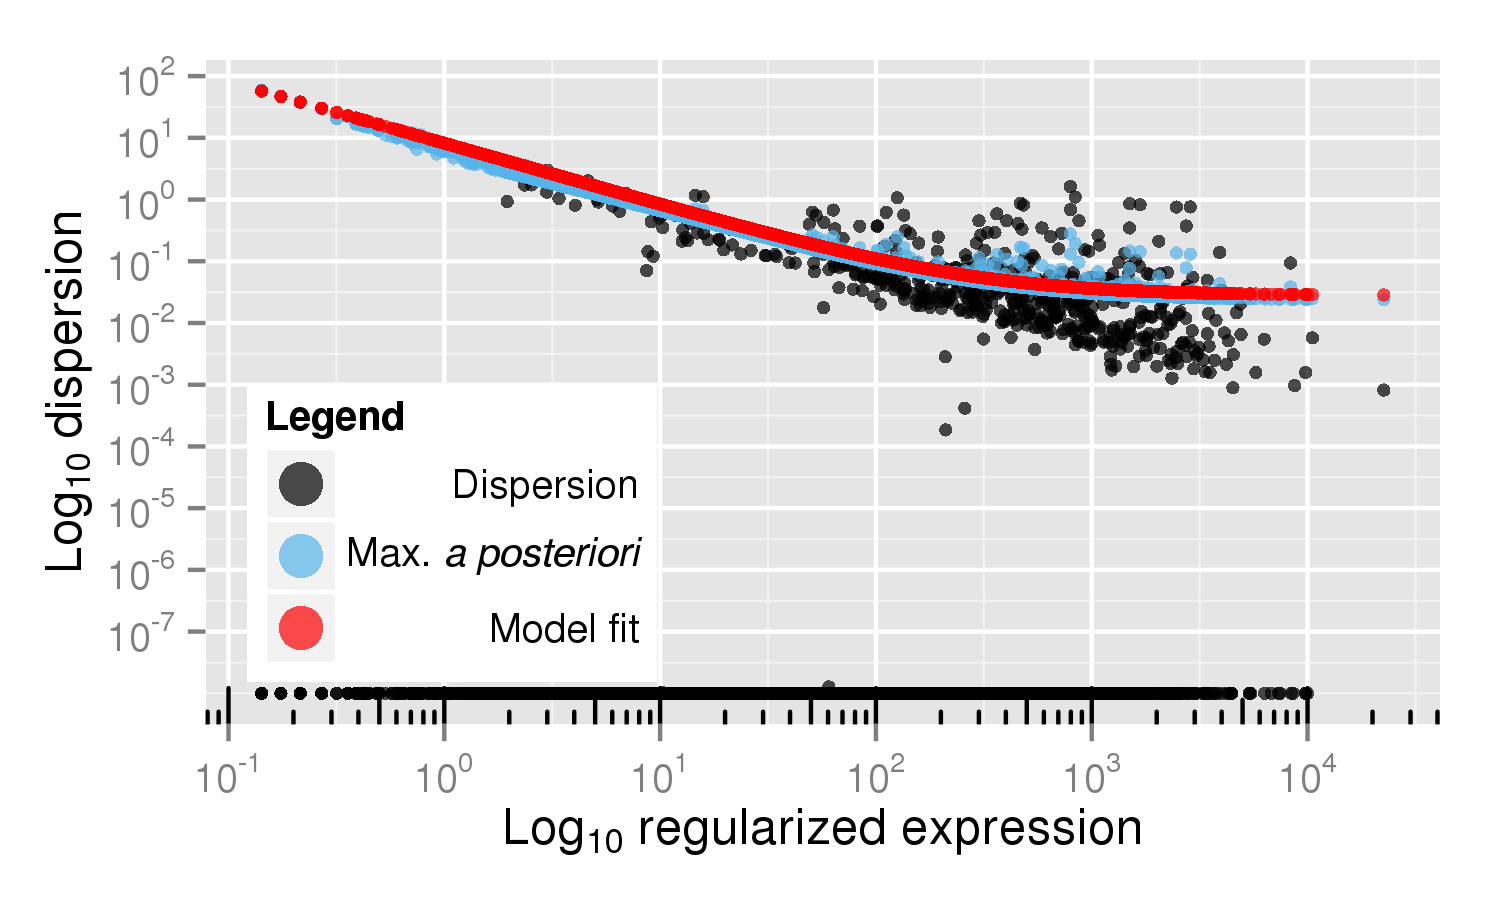
\includegraphics{images/Gene_dispersion}    % This file (results.tex) contains the text
                   % for Chapter 3- results


%					C H A P T E R   4 - Discussion
% This is the Chapter 4 - Discussion file (discussion.tex)

\chapter{Discussion}

    % This file (discussion.tex) contains the text
                   % for Chapter 4- discussion

%					C H A P T E R   5 - Conclusions


% This is the Chapter 5 - Conclusions file (conclusions.tex)

\chapter{Conclusions}

Renewables research revolves around the development of a feedstock-flexible chassis organism that requires minimal engineering for biofuels production, such as \textit{C. acetobutylicum}. The development of this organism requires a complete genome annotation consisting of ORFs, promoters, terminators, and transcript boundaries. The existing annotation of this microbe is largely the result of ORF predictions from antiquated gene models and is consequently incomplete. Genomic and molecular research will be more efficacious with an accurate genome annotation.

High-throughput transcriptomic methods such as RNA-seq are ideal to update this annotation, despite the well documented challenges related to this platform. Many of these challenges have not been addressed by the literature, leading to poor data utilization rates(Table \ref{table:study_compare}). The absence of standards for bacterial transcriptome mapping studies provided the opportunity to develop an innovative technique to explicitly address false positive and false negative signal in sequencing datasets.

Several problematic issues, including rRNA and RNA degradation, were addressed by developing a laboratory workflow and quality control system prior to deep sequencing. The dataset was cleaned for errors, biases, and contaminants for proper quantification of the sensitivity. 450M properly-paired reads provided \textgreater 9000 fold-coverage of the \textit{C. acetobutylicum}, with a median per-base sequencing depth of 156x. This method even detected low-level background signals, an issue affecting deep sequencing studies that leads to false positive errors, yet ignored by studies in the microbial community. 

To identify and treat these issues, a fast and flexible genome browser was constructed. The genome browser visualized the background signals and misassemblies that were detectable in assembly statistics. Genome-wide promoter predictions revealed the prevalence of $\sigma_{A}$-promoter elements in the AT-rich \textit{C. acetobutylicum} genome, a potential source for the background signals. An integrative analysis method was developed to correct the misassemblies where necessary by including sequencing depth, complexity, Rho-independent terminators, and promoter motifs in the annotation visualization and curation method.

Most examples required little to no curation and showed excellent precision and accuracy with respect to previous studies. Even challenging edge cases involving multiple transcription start sites had excellent signal to noise ratio and consequently simple corrections. A proof-of-principle curation of the pSOL1 megaplasmid produced ideal assembly statistics, including a median transcript size of 1.4kb consistent with the reported average transcript lengths in \textit{E. coli}. A total of 86 reference-ORF containing transcripts and 24 novel transcripts were identified.

By explicitly addressing several issues related to false positive and false negative signals, a sequencing protocol and integrative analysis method was developed. This method lead to the first strand-specific transcriptome assembly in the genus \textit{Clostridia}. The technique described by this work is applicable in any bacterial species where a genome sequence is available. While the unprecedented sequencing depth of this study lead to false positive results in the initial assembly, the integrative curation method provided both precision and accuracy in transcript boundary determination. 

\chapter{Future Work}
This study provided \textit{C. acetobutylicum} transcript boundaries for future molecular and genomics studies. The method used in the proof of principle curation of the pSOL1 megaplasmid should be extended to the entire \textit{C. acetobutylicum} chromosome. It is reasonable to expect that the transcript and UTR sizes for the whole genome should be similarly improved. The transcript boundaries could improve expression estimates and differential expression analyses. Beyond comparing with previous microarray studies, novel transcripts discovered here could be discovered to be stress responsive. Such findings would be natural targets for future targeted or whole genome stress response analyses. 

The transcript boundaries also facilitate regulatory motif identification. Besides the promoter motifs and transcription factor binding sites described here, new motifs could exist upstream of transcription start sites of clusters of co-regulated genes. Differential promoter usage can be investigated using the genome browser and gene-specific techniques. Gene networks in \textit{C. acetobutylicum} inevitably possess transcription activation systems and will be ready to be explored with a complete genome annotation.

In fact, differential expression and motif analyses can be combined in an interesting way. By coupling differentially expressed genes, their expression profiles, and clustering algorithms, patterns of co-expression and perhaps co-regulation may be identified. The performance of such an approach naturally depends on normalization approaches (to make profiles reasonably comparable) and clustering theory. While some approaches have been suggested for expression profiles specifically, the performance of any approach is ultimately determined by these two factors and thus all options should be explored. 

Additional research can be done with comparative genomics, including re-annotation of the genome and transcriptome for protein coding ORFs. With the example of the missing CAC2079 gene for example, there may be substantially transcribed and protein coding regions that require comparative analysis to identify metabolite exporters, two-component systems, and more. In fact, the RAST annotation system\cite{160} can be used to annotate transcriptomes, with some clever scripting and knowledge of its features.

Finally, additional analyses should be done for RNA hybridization and small RNA target prediction. Many recently identified stress responsive small RNAs\cite{39} have unknown targets and functions. Exploration of their roles has been prohibited by undefined UTR structures and thus the thermodynamics of interaction with their partners. A complete genome annotation provides these information and an additional tractable problem for \textit{C. acetobutylicum} researchers to explore.

The first assembly and annotation provided by this work presents a number of opportunities for additional work in \textit{C. acetobutylicum}. Increasing temperatures, CO$_{2}$ levels, and energy prices provide ethical and economical incentives to explore renewables research in this organism. A small number of intrinsic conditions have explored in this study, including the exponential and transition stages of growth, and stress responses to metabolite stress. Additional conditions may display alternate gene sets, expanding the complexity of the transcriptome beyond what is described here. Novel transcripts identified in the megaplasmid and chromosome require annotation and molecular study. If enzymes are discovered, metabolic models should be updated. Differential expression experiments are an increasingly useful method for understanding transcriptomic dynamics. Such studies in \textit{C. acetobutylicum} directly benefit from a wider and more complete genome annotation. This work facilitates future research in \textit{C. acetobutylicum} through the genome browser, which can incorporate future annotations and display expression data in a fast, flexible, and data-dense manner.



    % This file (conclusions.tex) contains the text
                   % for Chapter 5- conclusions


%					R E F E R E N C E S
%%
% This is the References file (ref.tex)
%
\renewcommand{\bibname}{References}
\begin{thereferences}
Lastname, Firstname  ``Title.''  \textit{Journal}, Year.

Lastname, Firstname, and Firstname Lastname.  \textit{Title of Book}.  Publisher, Year.
\end{thereferences}
      % This file (ref.tex) contains the text
                   % for the references.
                   
%%
% This is the Bibliography file (bib.tex)
%
% For 100-999 change 99 to 999; for 1000-9999 change 99 to 9999 
\begin{thebibliography}{99}
\bibitem{1}Lastname, Firstname  ``Title.''  \textit{Journal}, Year.

\bibitem{2}Lastname, Firstname, and Firstname Lastname.  \textit{Title of Book}.  Publisher, Year.
\end{thebibliography}
      % This file (bib.tex) contains the text
                   % for a bibliography.
                                      
%
% This is the Bibliography file (bibtex.tex)
% This generally works for BibTeX

% Use sample.bib for BibTeX database
%\phantomsection
%\addcontentsline{toc}{chapter}{ }
\renewcommand{\bibname}{BIBLIOGRAPHY}

\nocite{*}
\bibliography{endnote}{}
% BibTeX style (plain, alpha, unsrt)
\bibliographystyle{unsrt}



% N O T E: Make sure to convert back to endnote for Terry	 % This file (bibtex.tex) contains the text
                   % for a bibliography if using BibTeX with
                   % sample.bib
                                      
%%
% This is one Appendix file (app.tex)
%
\oneappendix{Title for Appendix}

This is the information for one appendix. This is to be used if there is only one appendix.      % This file (app.tex) contains the text
                   % for one Appendix. 

%			A P P E N D I X      A
%%
% This is the Appendix A file (appA.tex)
%
\appendix{Title of Appendix}

This is the information for the first appendix, Appendix A. Copy the base file, appA.tex, for each additional appendix needed such as appB.tex, appC.tex, etc. Modify the main base file to include each additional appendix file.

If there is only one appendix, then modify the main file to only use app.tex instead of appA.tex.     % This file (appA.tex) contains the text
                   % for Appendix A. 
 
 %			A P P E N D I X      B
%\include{appB}     % This file (appB.tex) contains the text
                   % for Appendix B.   
       
\end{document}